\documentclass[8pt]{beamer}
\usepackage[]{graphicx}
\usepackage[]{color}


\usetheme{metropolis}           % Use metropolis theme
\usepackage{amsmath}
\usepackage{mathrsfs}
\usepackage{tabularx}

\usepackage[style=authoryear]{biblatex}
\addbibresource{references.bib}
\usepackage{cleveref}
\renewcommand*{\bibfont}{\footnotesize}


\title{2023-24 Budget Proposals}
\author{Ryan Giordano}
\date{Apr 12th, 2023}
\institute{Children's Community Center}

\begin{document}


\def\subitem#1{\begin{itemize}\item #1\end{itemize}}


%%%%%%%%%%%%%%%%%%%%%%%%%%%%%%%%%%%%%%%%%%%%%%%%%%%%%%%%%%%%%%%%%%%%%%%
%%%%%%%%%%%%%%%%%%%%%%%%%%%%%%%%%%%%%%%%%%%%%%%%%%%%%%%%%%%%%%%%%%%%%%%
%%%%%%%%%%%%%%%%%%%%%%%%%%%%%%%%%%%%%%%%%%%%%%%%%%%%%%%%%%%%%%%%%%%%%%%

\begin{frame}{Outline}

%
\begin{itemize}
%
\item The recent history of the CCC budget.
\begin{itemize}
    \item Most of our expenses are staff, most of our income is tuition.
    \item We have kept expenses close to income to keep CCC accessible.
    \item We have arguably under-invested in teachers and buildings and grounds.
\end{itemize}
\pause
\item How did this year go financially?
\begin{itemize}
    \item Very well, due in large part to high aftercare enrollment.
    \item We approved two $\$50$k ``one-off'' expenses (a teacher bonus and hiring an architect)
    \item For next year, we adopted the expenses of equity tuition, but not the income.
\end{itemize}
\pause
\item Budget proposal scenarios:
\begin{itemize}
    \item ``Business as usual''
        \subitem{Tuition and salary increase with inflation only}
    \item ``Investing moderately''
        \subitem{Tuition increases 2\% over inflation}
    %
    \item ``Investing more heavily''
        \begin{itemize}
        %
        \item Tuition increases 4\% over inflation
        \item Teachers get 1\% raise over inflation
        %
        \end{itemize}
    %
    \item ``Optimistic business as usual''
        \begin{itemize}
        %
        \item Tuition increases with inflation only
        \item Teachers get 1\% raise over inflation
        \item Hope we get lucky with expenses \& other sources of income
        %
        \end{itemize}
%
\end{itemize}
\end{itemize}
%
\end{frame}


%%%%%%%%%%%%%%%%%%%%%%%%%%%%%%%%%%%%%%%%%%%%%%%%%%%%%%%%%%%%%%%%%%%%%%%
%%%%%%%%%%%%%%%%%%%%%%%%%%%%%%%%%%%%%%%%%%%%%%%%%%%%%%%%%%%%%%%%%%%%%%%
%%%%%%%%%%%%%%%%%%%%%%%%%%%%%%%%%%%%%%%%%%%%%%%%%%%%%%%%%%%%%%%%%%%%%%%

\begin{frame}{Where does our money come from, and what do we spend it on?}
%
Our income is almost all tuition, and our expenses are almost all salaries.

For example, in the 2018-2019 school year:
%
\begin{itemize}
%
\item Total income was $\sim$ \$594k
\begin{itemize}
    \item 91\% came from tuition ($\sim 2/3$ of this came from AM tuition)
    % \item 63\% came from AM tuition
    % \item 29\% came from ``contract care'' (PM1, PM2, etc.)
    % \item 8\% came from fees and donations
\end{itemize}
%
\item Total expenditures were $\sim$ \$568k
\begin{itemize}
    \item 87\% went to personnel
\end{itemize}
%
\end{itemize}
%
\pause
It is difficult to raise teachers' salaries without
raising tuition a comparable amount.

This led to our current policy on teacher raises and bonuses (PPM page 28):
%
\begin{itemize}
%
\item Teachers get an increase with inflation (``COLA''), but do not get raises.
\item  When we have a surplus we are supposed to:
\begin{itemize}
\item \textcolor{red}{Give teachers generous bonuses.}
\item \textcolor{red}{Fund the employee endowment fund (EEF).}
\end{itemize}
%
\end{itemize}
%

So how often / how much do we have surpluses?

% The first two years of COVID19 were different, as we will discuss later.
%
\end{frame}


%%%%%%%%%%%%%%%%%%%%%%%%%%%%%%%%%%%%%%%%%%%%%%%%%%%%%%%%%%%%%%%%%%%%%%%
%%%%%%%%%%%%%%%%%%%%%%%%%%%%%%%%%%%%%%%%%%%%%%%%%%%%%%%%%%%%%%%%%%%%%%%
%%%%%%%%%%%%%%%%%%%%%%%%%%%%%%%%%%%%%%%%%%%%%%%%%%%%%%%%%%%%%%%%%%%%%%%

\begin{frame}{Budget over time: pre-COVID19}
\begin{figure}
\begin{center}
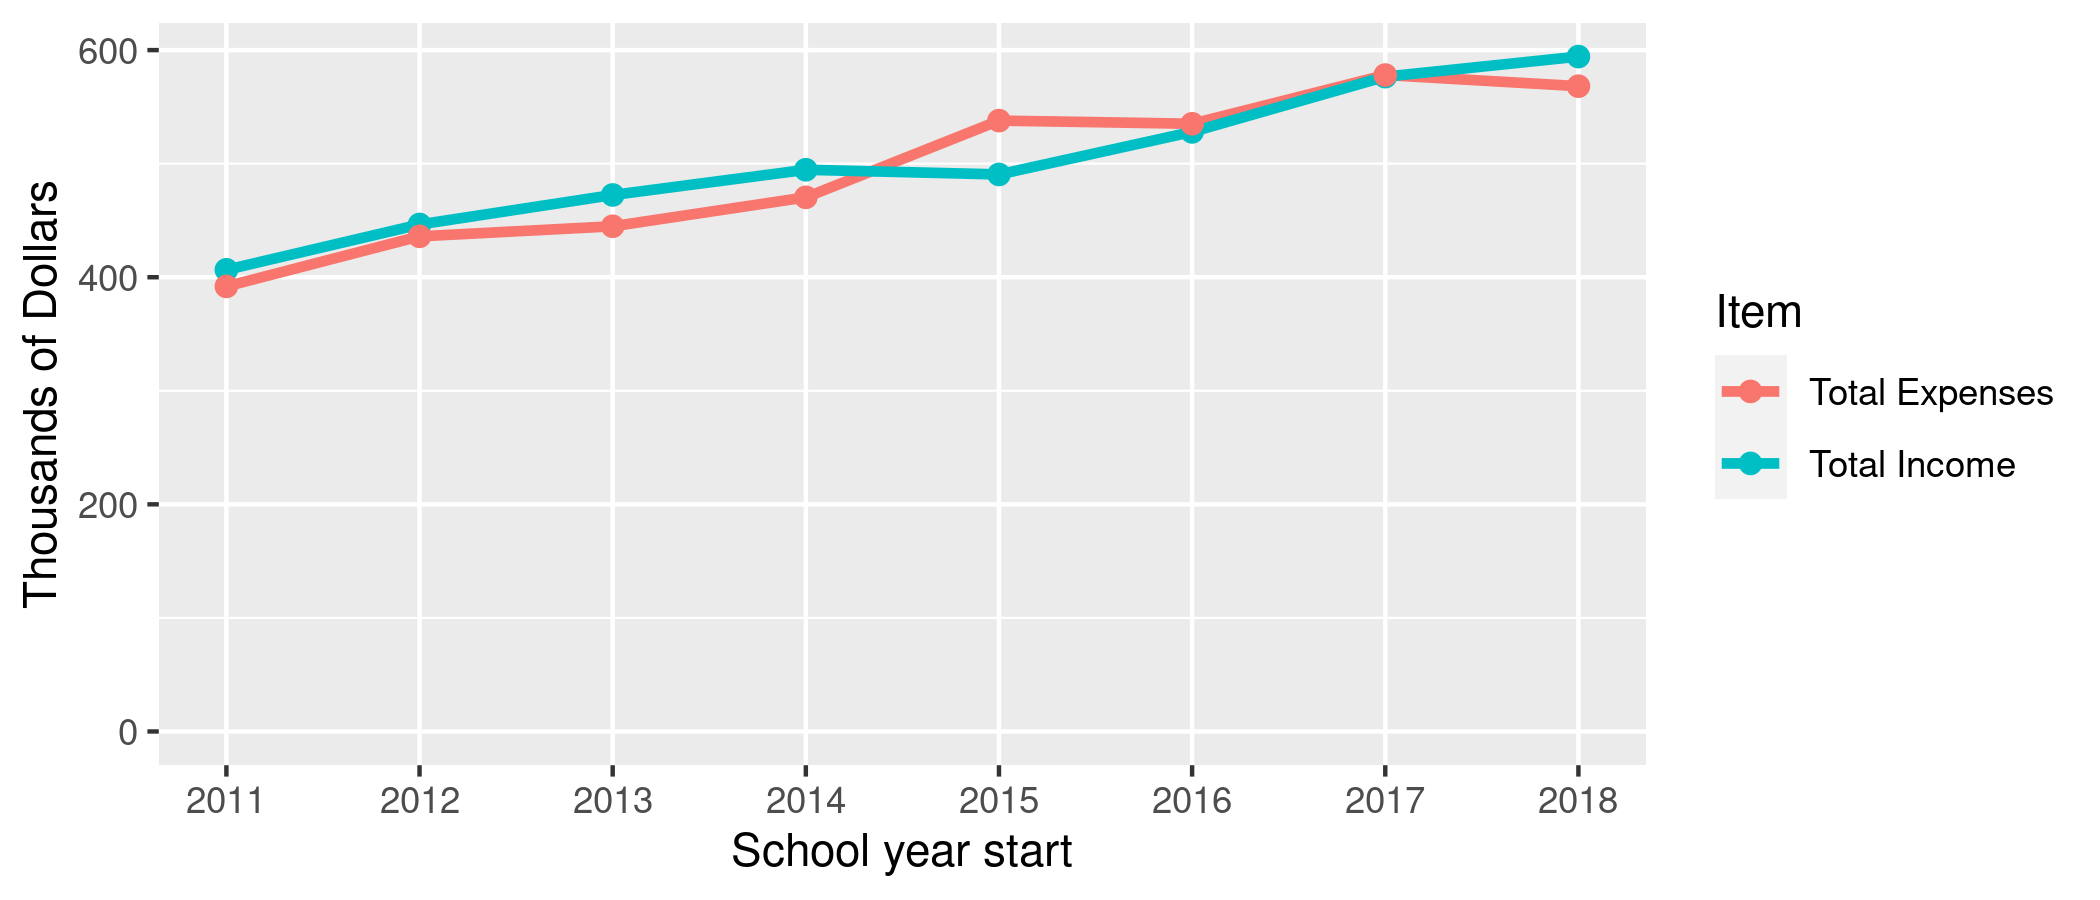
\includegraphics[width=3in]{budget_history.png}
\end{center}
\end{figure}

Between the 2011-2012 and 2018-2019 school years (inclusive):
%
\begin{itemize}
%
\item Actual income ran from $\sim$ \$400k - \$600k
\item The largest defecit was \$47k (10\%), and the largest surplus \$28k (4\%)
% \item These were 10\% and 4\% of revenue, respectively
\item Over all these years, the net surplus was \$47k ($\sim$\$6k or 1.2\% / year)
\item Typical variability was from a 0.5\% loss to 4.5\% surplus (IQR)
\item We met the budget 63\% of the time (5/8)
%
\end{itemize}
%
\textcolor{red}{Because we run a tight budget, we may have
under-invested in B\&G and teacher pay.}

\end{frame}


%%%%%%%%%%%%%%%%%%%%%%%%%%%%%%%%%%%%%%%%%%%%%%%%%%%%%%%%%%%%%%%%%%%%%%%
%%%%%%%%%%%%%%%%%%%%%%%%%%%%%%%%%%%%%%%%%%%%%%%%%%%%%%%%%%%%%%%%%%%%%%%
%%%%%%%%%%%%%%%%%%%%%%%%%%%%%%%%%%%%%%%%%%%%%%%%%%%%%%%%%%%%%%%%%%%%%%%


\begin{frame}{Budget over time: COVID19 years}
\begin{figure}
\begin{center}
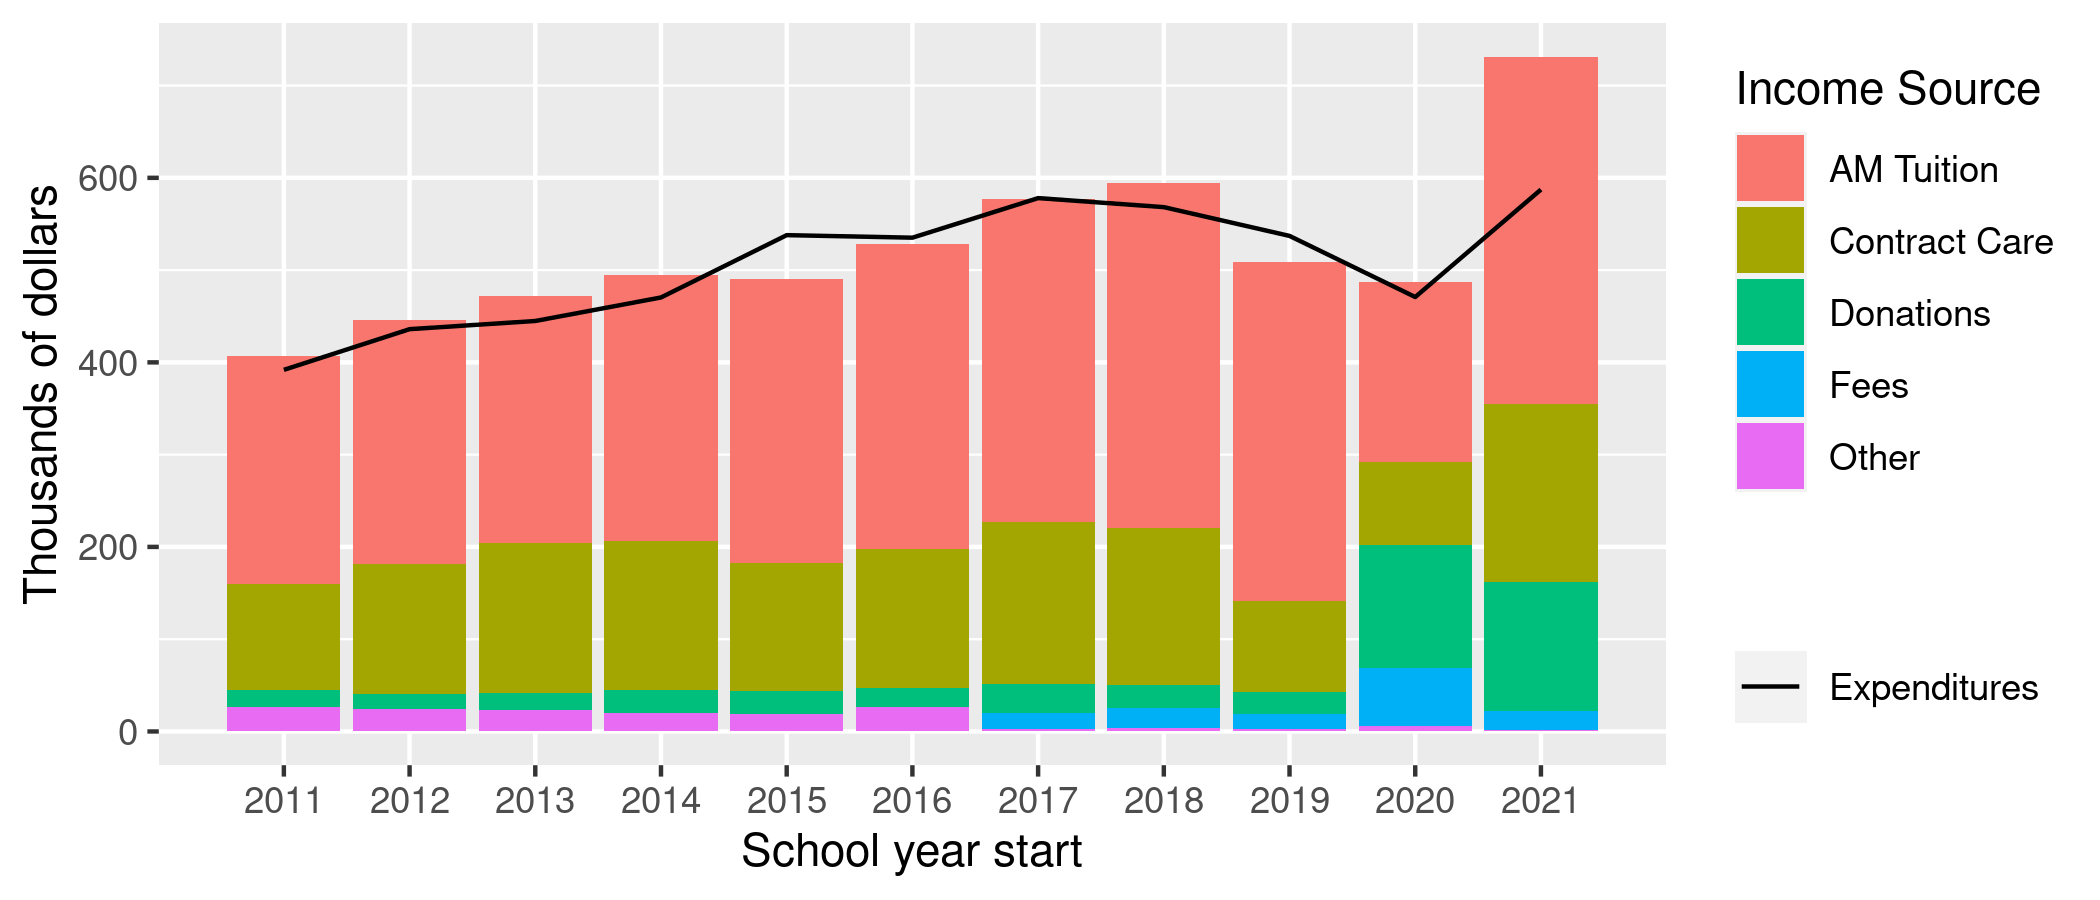
\includegraphics[width=3in]{budget_history_w_income_source.png}
\end{center}
\end{figure}

When COVID hit (midway through the 2019-2020 school year):
%
\begin{itemize}
%
\item We charged normal tuition for 2019-2020
\item Tuition dropped off steeply 2020-2021 (partial shutdown, fewer kids)
\item The shortfall was made up (and then some) from {\em one-time donations}:
\begin{itemize}
    \item Family donations
    \item Corporate donations
    \item Government assistance (in total over \$300k)
\end{itemize}
\item Without these donations, CCC would be close to out of business.
\item Instead, we emerged from COVID19 with a large, one-time surplus.
%
\end{itemize}
%
The surplus first went to the 20\% reserve.
\textbf{About \$278k remained last October.}.

Why didn't the teachers get a big bonus in 2021?  After subtracting one-time
donations, the surplus was only $\sim$\$5k, less than 1\% of budget.

\end{frame}


%%%%%%%%%%%%%%%%%%%%%%%%%%%%%%%%%%%%%%%%%%%%%%%%%%%%%%%%%%%%%%%%%%%%%%%
%%%%%%%%%%%%%%%%%%%%%%%%%%%%%%%%%%%%%%%%%%%%%%%%%%%%%%%%%%%%%%%%%%%%%%%
%%%%%%%%%%%%%%%%%%%%%%%%%%%%%%%%%%%%%%%%%%%%%%%%%%%%%%%%%%%%%%%%%%%%%%%

\begin{frame}{How did we do this year?}


\textbf{How did we use the surplus?}

About \$278k remained at the start of the year.
Currently, about \$202k remains.

(Not counting reserve reserve or CD funds.)

%
\begin{enumerate}
%
\item Operating expenses increased, so our reserve requirement increased.
\item Gave the teachers a bonus / funding the employee endowment fund
\subitem{One-time \$50k bonus and contribution to employee endowment fund}
%
\end{enumerate}

\textbf{How were our finances otherwise?}

Our finances were pretty good this year!

%
\begin{itemize}
%
\item As of March 1st, we were net $\$27$k positive
\subitem{Even including the one-time teacher bonus!}
\item Good finances were driven by high PM enrollment and hiring Lillian.
%
\end{itemize}
%


%
\end{frame}

%%%%%%%%%%%%%%%%%%%%%%%%%%%%%%%%%%%%%%%%%%%%%%%%%%%%%%%%%%%%%%%%%%%%%%%
%%%%%%%%%%%%%%%%%%%%%%%%%%%%%%%%%%%%%%%%%%%%%%%%%%%%%%%%%%%%%%%%%%%%%%%
%%%%%%%%%%%%%%%%%%%%%%%%%%%%%%%%%%%%%%%%%%%%%%%%%%%%%%%%%%%%%%%%%%%%%%%


\begin{frame}{What is coming next year?}

%
\begin{enumerate}
%
\item Inflation (COLA) is 4.9\% year over year.
\subitem{Tuition and salaries will increase by at least this amount.}
\pause
\item Potential decrease in PM enrollment (we got lucky this year)
\pause
\item Investing in buildings and grounds
%
    \begin{itemize}
    %
    \item Proposed \$5k for painting, \$50k for architect.
    \item \textcolor{red}{Currently not funded from tuition.}
    %
    \end{itemize}
%
\pause
\item Jump-starting ``equity tuition''
    %
    \begin{itemize}
    %
    \item Increases in scholarships to new families
    \item Equity tuition prices offered to families who would have had their
    tuition reduced
    \item ...but families who would have their tuition increased are still paying
    the same.
    \item Total projected scholarship cost next year $\$54$k (vs $\$23$k last year).
    \item There is a special fundraiser aiming to raise $\$60$k (currently
    raised $\$20$k).
    \item \textcolor{red}{Currently not funded from tuition.}
    %
    \end{itemize}
%
\item Changes to admin staff
\pause
    \begin{itemize}
        \item Currently, Edna works 32 hours per week, but got evicted and had to move out of state.
        \item Devaki is training to replace her, but cannot work more than 20 hours per week.
        \item Hire someone else?  Retain Edna?  Parent volunteers?  Need more than 32 hours?
    \end{itemize}
%
\item Teacher raises
\pause
    \begin{itemize}
        \item The bonus was a good thing to do, but arguably was making up for the past.
        \item There is some support for salary increases as well.
        \item \textcolor{red}{Currently not funded from tuition.}
    \end{itemize}
\end{enumerate}
%
\pause
\textbf{Should we deplete reserves for teacher bonuses, B\&G, and scholarships?}\\
\textbf{Or should we fund them, at least in part, with tuition increases?}

\end{frame}


\begin{frame}{Budget scenarios}
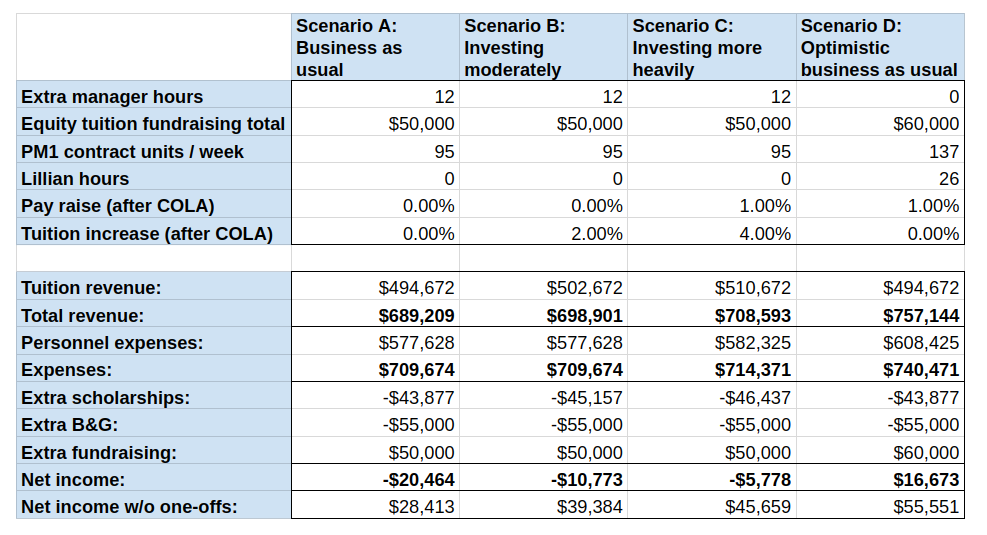
\includegraphics[width=4in]{budget_scenarios.png}

\end{frame}

\end{document}
